\documentclass{report}

\title{Adigraph, \AdigraphVersionNumber}
\author{Luca Cappelletti}
\date{December 2018}

\usepackage{adigraph}
\usepackage{xcolor}
\usepackage[colorlinks=true,urlcolor=blue,pdfpagelabels,hyperindex=false]{hyperref}
\usepackage{minted}
\usepackage{multicol}
\usepackage{graphicx} % for images and generally graphics
\usepackage{caption} % enabling of nice captions
\usepackage{subcaption} % and subcaptions of images
\definecolor{mintedbackground}{rgb}{0.95,0.95,0.95}
\setminted{
  bgcolor=mintedbackground,
  fontfamily=tt,
  linenos=true,
  numberblanklines=true,
  numbersep=5pt,
  gobble=0,
  frame=leftline,
  framerule=0.4pt,
  framesep=2mm,
  funcnamehighlighting=true,
  tabsize=4,
  obeytabs=false,
  mathescape=false
  samepage=false, %with this setting you can force the list to appear on the same page
  showspaces=false,
  showtabs =false,
  texcl=false,
}

%%%%%%%%%%%%%%%%%%%%%%%%%%%%%%%%%%%%%%%%%%%%%%%%%%%%%%%%%
% THE FOLLOWING CENTERS ALL FLOATING ITEMS BY DEFAULT   %
%%%%%%%%%%%%%%%%%%%%%%%%%%%%%%%%%%%%%%%%%%%%%%%%%%%%%%%%%

\makeatletter
\g@addto@macro\@floatboxreset\centering
\makeatother

\makeatletter
\apptocmd\subcaption@minipage{\centering}{}{}
\makeatother

\makeatletter
\providecommand*\setfloatlocations[2]{\@namedef{fps@#1}{#2}}
\makeatother
\setfloatlocations{figure}{H}
\setfloatlocations{table}{H}

\begin{document}

\maketitle

{\hypersetup{hidelinks}
	\tableofcontents  % Generates the table of contents
}

\chapter{Introduction}
\section{What is Adigraph?}
\textbf{\href{https://ctan.org/pkg/adigraph}{Adigraph}} is a latex library for drawing directed graphs and augmenting directed graphs, and to draw cuts over them.

It handles automatically the positioning of labels, with the exception of the horizontal position, and the inclinations of cuts.

The latest version is available on \href{https://github.com/LucaCappelletti94/adigraph}{Github}.

\section{License}
Copyright 2018 Luca Cappelletti

Permission is hereby granted, free of charge, to any person obtaining a copy of this software and associated documentation files (the "Software"), to deal in the Software without restriction, including without limitation the rights to use, copy, modify, merge, publish, distribute, sub-license, and/or sell copies of the Software, and to permit persons to whom the Software is furnished to do so, subject to the following conditions:

The above copyright notice and this permission notice shall be included in all copies or substantial portions of the Software.

THE SOFTWARE IS PROVIDED "AS IS", WITHOUT WARRANTY OF ANY KIND, EXPRESS OR IMPLIED, INCLUDING BUT NOT LIMITED TO THE WARRANTIES OF MERCHANTABILITY, FITNESS FOR A PARTICULAR PURPOSE AND NONINFRINGEMENT. IN NO EVENT SHALL THE AUTHORS OR COPYRIGHT HOLDERS BE LIABLE FOR ANY CLAIM, DAMAGES OR OTHER LIABILITY, WHETHER IN AN ACTION OF CONTRACT, TORT OR OTHERWISE, ARISING FROM, OUT OF OR IN CONNECTION WITH THE SOFTWARE OR THE USE OR OTHER DEALINGS IN THE SOFTWARE.\\

\chapter{Setup}
\section{Installing the dependencies}
Clearly you need to have texlive installed. Then, make sure you have the following packages:

\begin{description}
	\item[\href{https://ctan.org/pkg/fp}{fp}] Used for floating point calculations.
	\item[\href{https://ctan.org/pkg/xparse}{xparse}] Used for elaborating parameters.
	\item[\href{https://ctan.org/pkg/xstring}{xstring}] Used for elaborating strings.
	\item[\href{https://ctan.org/pkg/etoolbox}{etoolbox}] Used for operations on lists.
	\item[tikz] Used for drawing the actual graphs.
	\item[tikz calc library] Used for some internal calculations in tikz.
\end{description}

To be sure you can run the following, that will install the packages only if they are not already present:

\begin{minted}{sh}
sudo tlmgr install etoolbox fp xstring
\end{minted}

\section{Installing Adigraph}
You can install Adigraph, if it isn't already present in your setup, by running the following on Unix systems:

\begin{minted}{sh}
sudo tlmgr install adigraph
\end{minted}

On windows you should check on your package manager of choice (some latex distribution have a tlmgr implementation on windows too.)

\chapter{Usage}
\section{Creating a new graph}
Here we create a new Adigraph object, called \textit{myAdigraph}.

\begin{minted}{latex}
\NewAdigraph{myAdigraph}{
	<nodes here, separated by semicolon>
}{
	<edges here, separated by semicolon>
}{
	<cuts here, separated by semicolon>
}[
	<edge style here>
]
\end{minted}

\section{Changing an existing graph}
You can renovate an older graph by calling \textbackslash RenewAdigraph

\begin{minted}{latex}
\RenewAdigraph{myAdigraph}{
	<nodes here, separated by semicolon>
}{
	<edges here, separated by semicolon>
}{
	<cuts here, separated by semicolon>
}[
	<edge style here>
]
\end{minted}

\section{Adding nodes}
We set its nodes with the following syntax: \textit{<node name[, textual color, border width]: \(x\) coordinate[, \(y\) coordinate][: label]>}.

\begin{figure}
	\begin{subfigure}{0.49\textwidth}
		\begin{minted}{latex}
\NewAdigraph{myAdigraph}{
 	s:0,0;
 	t:4,0;
}
\myAdigraph{}
\end{minted}
	\end{subfigure}
	\begin{subfigure}{0.49\textwidth}
		\NewAdigraph{myAdigraph}{
			s:0,0;
			t:4,0;
		}
		\myAdigraph{}
	\end{subfigure}
\end{figure}

\subsection{Custom node colors}
To color a node you can use the following syntax: \textit{<node name[, textual color]: \(x\) coordinate[, \(y\) coordinate]>}. For example, to draw s in red and t in blue we would write:

\begin{figure}
	\begin{subfigure}{0.49\textwidth}
		\begin{minted}{latex}
\NewAdigraph{myAdigraph}{
 	s,red:0,0;
 	t,blue:4,0;
}
\myAdigraph{}
\end{minted}
	\end{subfigure}
	\begin{subfigure}{0.49\textwidth}
		\NewAdigraph{myAdigraph}{
			s,red:0,0;
			t,blue:4,0;
		}
		\myAdigraph{}
	\end{subfigure}
\end{figure}

Tested available colors are: red, blue, black, green. You may extend the possible colors with LaTex libraries such as xcolor.

\subsection{Custom node width}
To color a node you can use the following syntax: \textit{<node name[, textual color[, border width]]: \(x\) coordinate[, \(y\) coordinate]>}. For example:

\begin{figure}
	\begin{subfigure}{0.49\textwidth}
		\begin{minted}{latex}
\NewAdigraph{myAdigraph}{
 	s,red,5:0,0;
 	t,blue,3:4,0;
}
\myAdigraph{}
\end{minted}
	\end{subfigure}
	\begin{subfigure}{0.49\textwidth}
		\NewAdigraph{myAdigraph}{
			s,red,5:0,0;
			t,blue,3:4,0;
		}
		\myAdigraph{}
	\end{subfigure}
\end{figure}

\subsection{Custom node labels}
To add a custom label you can use the following syntax: either \textit{<node name: \(x\) coordinate[, \(y\) coordinate][: node label]>} or \textit{<node name[, textual color]: \(x\) coordinate[, \(y\) coordinate][: node label]>} will work:

\begin{figure}
	\begin{subfigure}{0.49\textwidth}
		\begin{minted}{latex}
\NewAdigraph{myAdigraph}{
 	s,red:0,0:start;
 	t:4,0:end;
}
\myAdigraph{}
\end{minted}
	\end{subfigure}
	\begin{subfigure}{0.49\textwidth}
		\NewAdigraph{myAdigraph}{
			s,red:0,0:start;
			t:4,0:end;
		}
		\myAdigraph{}
	\end{subfigure}
\end{figure}

\section{Automatically position nodes}
When no coordinates are given or you just don't have time to think about where to put those nodes, just choose a radius and Adigraph will position them on the circle of that radius.

\begin{figure}
	\begin{subfigure}{0.49\textwidth}
		\begin{minted}{latex}
\NewAdigraph{myAdigraph}{
	1:0,0;
	2:2;
	3:2;
	4:2;
	5:2;
	6:2;
	7:2;
	8:2;
}
\myAdigraph{}
\end{minted}
	\end{subfigure}
	\begin{subfigure}{0.49\textwidth}
		\NewAdigraph{myAdigraph}{
			1:0,0;
			2:2;
			3:2;
			4:2;
			5:2;
			6:2;
			7:2;
			8:2;
		}
		\myAdigraph{}
	\end{subfigure}
\end{figure}

\subsection{Colored automatically positioned nodes}

\begin{figure}
	\begin{subfigure}{0.49\textwidth}
		\begin{minted}{latex}
\NewAdigraph{myAdigraph}{
	1:0,0;
	2,purple:2;
	3,brown:2;
	4,gray:2;
	5,blue:2;
	6,red:2;
	7,green:2;
	8,pink:2;
}
\myAdigraph{}
\end{minted}
	\end{subfigure}
	\begin{subfigure}{0.49\textwidth}
		\NewAdigraph{myAdigraph}{
			1:0,0;
			2,purple:2;
			3,brown:2;
			4,gray:2;
			5,blue:2;
			6,red:2;
			7,green:2;
			8,pink:2;
		}
		\myAdigraph{}
	\end{subfigure}
\end{figure}


\section{Adding edges}
We set its edges with the following syntax: \textit{<first node, second node,[color,[edge width]][:weight[:label:[label position]]]>}.

\subsection{A simple edge}
\begin{figure}
	\begin{subfigure}{0.49\textwidth}
		\begin{minted}{latex}
\NewAdigraph{myAdigraph}{
 	s:0,0;
 	t:4,0;
}{
	s,t;
}
\myAdigraph{}
\end{minted}
	\end{subfigure}
	\begin{subfigure}{0.49\textwidth}
		\NewAdigraph{myAdigraph}{
			s:0,0;
			t:4,0;
		}{
			s,t;
		}
		\myAdigraph{}
	\end{subfigure}
\end{figure}

\subsection{A looped edge}
Looped edges position automatically by themselves to minimize overlapping.
\begin{figure}
	\begin{subfigure}{0.49\textwidth}
		\begin{minted}{latex}
\NewAdigraph{myAdigraph}{
 	s:0,0;
 	t:4,0;
}{
	s,s;
	t,t;
	s,t;
}
\myAdigraph{}
\end{minted}
	\end{subfigure}
	\begin{subfigure}{0.49\textwidth}
		\NewAdigraph{myAdigraph}{
			s:0,0;
			t:4,0;
		}{
			s,s;
			t,t;
			s,t;
		}
		\myAdigraph{}
	\end{subfigure}
\end{figure}

\subsection{A colored simple edge}
\begin{figure}
	\begin{subfigure}{0.49\textwidth}
		\begin{minted}{latex}
\NewAdigraph{myAdigraph}{
 	s:0,0;
 	t:4,0;
}{
	s,t,red;
}
\myAdigraph{}
\end{minted}
	\end{subfigure}
	\begin{subfigure}{0.49\textwidth}
		\NewAdigraph{myAdigraph}{
			s:0,0;
			t:4,0;
		}{
			s,t,red;
		}
		\myAdigraph{}
	\end{subfigure}
\end{figure}

\subsection{A wider simple edge}
\begin{figure}
	\begin{subfigure}{0.49\textwidth}
		\begin{minted}{latex}
\NewAdigraph{myAdigraph}{
 	s:0,0;
 	t:4,0;
}{
	s,t,red,5;
}
\myAdigraph{}
\end{minted}
	\end{subfigure}
	\begin{subfigure}{0.49\textwidth}
		\NewAdigraph{myAdigraph}{
			s:0,0;
			t:4,0;
		}{
			s,t,red,5;
		}
		\myAdigraph{}
	\end{subfigure}
\end{figure}

\subsection{A weighted edge}
\begin{figure}
	\begin{subfigure}{0.49\textwidth}
		\begin{minted}{latex}
\NewAdigraph{myAdigraph}{
 	s:0,0;
 	t:4,0;
}{
	s,t:56;
}
\myAdigraph{}
\end{minted}
	\end{subfigure}
	\begin{subfigure}{0.49\textwidth}
		\NewAdigraph{myAdigraph}{
			s:0,0;
			t:4,0;
		}{
			s,t:56;
		}
		\myAdigraph{}
	\end{subfigure}
\end{figure}

\subsection{A weighted edge with label}
\begin{figure}
	\begin{subfigure}{0.49\textwidth}
		\begin{minted}{latex}
\NewAdigraph{myAdigraph}{
 	s:0,0;
 	t:4,0;
}{
	s,t:56:myLabel;
}
\myAdigraph{}
\end{minted}
	\end{subfigure}
	\begin{subfigure}{0.49\textwidth}
		\NewAdigraph{myAdigraph}{
			s:0,0;
			t:4,0;
		}{
			s,t:56:myLabel;
		}
		\myAdigraph{}
	\end{subfigure}
\end{figure}

\subsection{Edge in both directions}
\begin{figure}
	\begin{subfigure}{0.49\textwidth}
		\begin{minted}{latex}
\NewAdigraph{myAdigraph}{
 	s:0,0;
 	t:4,0;
}{
	s,t;
	t,s;
}
\myAdigraph{}
\end{minted}
	\end{subfigure}
	\begin{subfigure}{0.49\textwidth}
		\NewAdigraph{myAdigraph}{
			s:0,0;
			t:4,0;
		}{
			s,t;
			t,s;
		}
		\myAdigraph{}
	\end{subfigure}
\end{figure}

\subsection{Edge with weights in both directions}
\begin{figure}
	\begin{subfigure}{0.49\textwidth}
		\begin{minted}{latex}
\NewAdigraph{myAdigraph}{
 	s:0,0;
 	t:4,0;
}{
	s,t:5;
	t,s:5;
}
\myAdigraph{}
\end{minted}
	\end{subfigure}
	\begin{subfigure}{0.49\textwidth}
		\NewAdigraph{myAdigraph}{
			s:0,0;
			t:4,0;
		}{
			s,t:5;
			t,s:5;
		}
		\myAdigraph{}
	\end{subfigure}
\end{figure}

\subsection{Positioning labels}
\begin{figure}
	\begin{subfigure}{0.49\textwidth}
		\begin{minted}{latex}
\NewAdigraph{myAdigraph}{
	1:0,0;
	2:0,2;
	3:4,2;
	4:4,0;
}{
	1,3,red:1:a:near start;
	2,4,blue:1:b:near end;
}
\myAdigraph{}
\end{minted}
	\end{subfigure}
	\begin{subfigure}{0.49\textwidth}
		\NewAdigraph{myAdigraph}{
			1:0,0;
			2:0,2;
			3:4,2;
			4:4,0;
		}{
			1,3,red:1:a:near start;
			2,4,blue:1:b:near end;
		}
		\myAdigraph{}
	\end{subfigure}
\end{figure}

\subsection{Positioning weights}
\begin{figure}
	\begin{subfigure}{0.49\textwidth}
		\begin{minted}{latex}
\NewAdigraph{myAdigraph}{
	1:0,0;
	2:0,2;
	3:4,2;
	4:4,0;
}{
	1,3,red:1::near start;
	2,4,blue:1::near end;
}
\myAdigraph{}
\end{minted}
	\end{subfigure}
	\begin{subfigure}{0.49\textwidth}
		\NewAdigraph{myAdigraph}{
			1:0,0;
			2:0,2;
			3:4,2;
			4:4,0;
		}{
			1,3,red:1::near start;
			2,4,blue:1::near end;
		}
		\myAdigraph{}
	\end{subfigure}
\end{figure}


\subsection{Multiple edges with weights}
\begin{figure}
	\begin{subfigure}{0.49\textwidth}
		\begin{minted}{latex}
\NewAdigraph{myAdigraph}{
	s:0,0;
	t:4,0;
	1:0,3;
	2:4,3;
}{
	s,t:5;
	t,s:5;
	s,1:5;
	1,s:5;
	1,2:5;
	2,1:5;
	2,t:5;
	t,2:5;
	t,1:5;
	1,t:5;
}
\myAdigraph{}
\end{minted}
	\end{subfigure}
	\begin{subfigure}{0.49\textwidth}
		\NewAdigraph{myAdigraph}{
			s:0,0;
			t:4,0;
			1:0,3;
			2:4,3;
		}{
			s,t:5;
			t,s:5;
			s,1:5;
			1,s:5;
			1,2:5;
			2,1:5;
			2,t:5;
			t,2:5;
			t,1:5;
			1,t:5;
		}
		\myAdigraph{}
	\end{subfigure}
\end{figure}

\section{Kleene star operators}
\subsection{Kleene star on an element}
This works only when you don't have a node called \textit{<*>}. When this happens, the behaviour of a tuple \textit{<a,*>} becomes the normal one.
\begin{figure}
	\begin{subfigure}{0.49\textwidth}
		\begin{minted}{latex}
\NewAdigraph{myAdigraph}{
	1:3;
	2:3;
	3:3;
	4:3;
	5:3;
	6:3;
	7:3;
	8:3;
}{
	1,*,blue;
	*,4,red;
}
\myAdigraph{}
\end{minted}
	\end{subfigure}
	\begin{subfigure}{0.49\textwidth}
		\NewAdigraph{myAdigraph}{
			1:3;
			2:3;
			3:3;
			4:3;
			5:3;
			6:3;
			7:3;
			8:3;
		}{
			1,*,blue;
			*,4,red;
		}
		\myAdigraph{}
	\end{subfigure}
\end{figure}

\subsection{Kleene star minus the element}
This works only when you don't have a node called \textit{<+>}. When this happens, the behaviour of a tuple \textit{<a,+>} becomes the normal one.
\begin{figure}
	\begin{subfigure}{0.49\textwidth}
		\begin{minted}{latex}
\NewAdigraph{myAdigraph}{
	1:3;
	2:3;
	3:3;
	4:3;
	5:3;
	6:3;
	7:3;
	8:3;
}{
	1,+,blue;
	+,4;
}
\myAdigraph{}
\end{minted}
	\end{subfigure}
	\begin{subfigure}{0.49\textwidth}
		\NewAdigraph{myAdigraph}{
			1:3;
			2:3;
			3:3;
			4:3;
			5:3;
			6:3;
			7:3;
			8:3;
		}{
			1,+,blue;
			+,4;
		}
		\myAdigraph{}
	\end{subfigure}
\end{figure}


\subsection{Combining Kleene operations}
Sadly, operations such as \textit{<*,+>} or \textit{<+,+>} are not currently supported and not for lack of trying. I'll try implementing them again in the future when I'll have more time.

\section{Paths}
A path is specified by the following syntax: \textit{<comma separated list of nodes>}.

\NewAdigraph{myPathsTestAdigraph}{
	s:0,0;
	1:2,2;
	3:2,-2;
	2:6,2;
	4:6,-2;
	t:8,0;
}{
	s,1:25;
	s,3:25;
	3,4:25;
	1,2:35;
	2,t:20;
	4,t:30;
	3,1:10;
	4,2:10;
	2,3:15::near start;
	4,1:5::near start;
}

\begin{figure}
	\begin{subfigure}{0.49\textwidth}
		\begin{minted}{latex}
\NewAdigraph{myAdigraph}{
	s:0,0;
	1:2,2;
	3:2,-2;
	2:6,2;
	4:6,-2;
	t:8,0;
}{
	s,1:25;
	s,3:25;
	3,4:25;
	1,2:35;
	2,t:20;
	4,t:30;
	3,1:10;
	4,2:10;
	2,3:15::near start;
	4,1:5::near start;
}
\myAdigraph{
	s,3,4,2,t;
}
\end{minted}
	\end{subfigure}
	\begin{subfigure}{0.49\textwidth}
		\myPathsTestAdigraph{
			s,3,4,2,t;
		}
	\end{subfigure}
\end{figure}

\subsection{Augmenting paths}
An augmenting path is specified by the following syntax: \textit{<comma separated list of nodes:units>}. It is \textbf{very important} to note that incremental paths called upon the same object are memorized by default.

\NewAdigraph{myAdigraph}{
	s:0,0;
	1:2,2;
	3:2,-2;
	2:6,2;
	4:6,-2;
	t:8,0;
}{
	s,1:25;
	s,3:25;
	3,4:25;
	1,2:35;
	2,t:20;
	4,t:30;
	3,1:10;
	4,2:10;
	2,3:15::near start;
	4,1:5::near start;
}

\begin{figure}
	\begin{subfigure}{0.49\textwidth}
		\begin{minted}{latex}
\NewAdigraph{myAdigraph}{
	s:0,0;
	1:2,2;
	3:2,-2;
	2:6,2;
	4:6,-2;
	t:8,0;
}{
	s,1:25;
	s,3:25;
	3,4:25;
	1,2:35;
	2,t:20;
	4,t:30;
	3,1:10;
	4,2:10;
	2,3:15::near start;
	4,1:5::near start;
}
\myAdigraph{
	s,3,4,2,t:5;
}
\end{minted}
	\end{subfigure}
	\begin{subfigure}{0.49\textwidth}
		\myAdigraph{
			s,3,4,2,t:5;
		}
	\end{subfigure}
\end{figure}

For example, suppose now we'd like to send another 5 units on the graph edited by the previous incremental path, we'll have just to write the following:

\begin{figure}
	\begin{subfigure}{0.49\textwidth}
		\begin{minted}{latex}
\myAdigraph{
	s,3,4,1,2,t:5;
}
\end{minted}
	\end{subfigure}
	\begin{subfigure}{0.49\textwidth}
		\myAdigraph{
			s,3,4,1,2,t:5;
		}
	\end{subfigure}
\end{figure}

\begin{figure}
	\begin{subfigure}{0.49\textwidth}
		\begin{minted}{latex}
\myAdigraph{
	s,3,4,t:15;
}
\end{minted}
	\end{subfigure}
	\begin{subfigure}{0.49\textwidth}
		\myAdigraph{
			s,3,4,t:15;
		}
	\end{subfigure}
\end{figure}

\begin{figure}
	\begin{subfigure}{0.49\textwidth}
		\begin{minted}{latex}
\myAdigraph{
	s,1,4,t:5;
}
\end{minted}
	\end{subfigure}
	\begin{subfigure}{0.49\textwidth}
		\myAdigraph{
			s,1,4,t:5;
		}
	\end{subfigure}
\end{figure}

\begin{figure}
	\begin{subfigure}{0.49\textwidth}
		\begin{minted}{latex}
\myAdigraph{
	s,1,2,t:10;
}
\end{minted}
	\end{subfigure}
	\begin{subfigure}{0.49\textwidth}
		\myAdigraph{
			s,1,2,t:10;
		}
	\end{subfigure}
\end{figure}

\begin{figure}
	\begin{subfigure}{0.49\textwidth}
		\begin{minted}{latex}
\myAdigraph{
	s,1,2,4,t:5;
}
\end{minted}
	\end{subfigure}
	\begin{subfigure}{0.49\textwidth}
		\myAdigraph{
			s,1,2,4,t:5;
		}
	\end{subfigure}
\end{figure}

\subsection{Custom colored augmenting Paths}
A path is specified by the following syntax: \textit{<comma separated list of nodes>:<units>:<forward path color, backward path color>}.

\NewAdigraph{myCustomAugmentingPathAdigraph}{
	s:0,0;
	1:2,2;
	3:2,-2;
	2:6,2;
	4:6,-2;
	t:8,0;
}{
	s,1:25;
	s,3:25;
	3,4:25;
	1,2:35;
	2,t:20;
	4,t:30;
	3,1:10;
	4,2:10;
	2,3:15::near start;
	4,1:5::near start;
}

\begin{figure}
	\begin{subfigure}{0.49\textwidth}
		\begin{minted}{latex}
\NewAdigraph{myAdigraph}{
	s:0,0;
	1:2,2;
	3:2,-2;
	2:6,2;
	4:6,-2;
	t:8,0;
}{
	s,1:25;
	s,3:25;
	3,4:25;
	1,2:35;
	2,t:20;
	4,t:30;
	3,1:10;
	4,2:10;
	2,3:15::near start;
	4,1:5::near start;
}
\myAdigraph{
	s,3,4,2,t:5:green,blue;
}
\end{minted}
	\end{subfigure}
	\begin{subfigure}{0.49\textwidth}
		\myCustomAugmentingPathAdigraph{
			s,3,4,2,t:5:green,blue;
		}
	\end{subfigure}
\end{figure}

\subsection{Custom colored Paths}
A path is specified by the following syntax: \textit{<comma separated list of nodes>::<forward path color, backward path color>}. \textbf{Note the double colons!}.

\NewAdigraph{myCustomPathAdigraph}{
	s:0,0;
	1:2,2;
	3:2,-2;
	2:6,2;
	4:6,-2;
	t:8,0;
}{
	s,1:25;
	s,3:25;
	3,4:25;
	1,2:35;
	2,t:20;
	4,t:30;
	3,1:10;
	4,2:10;
	2,3:15::near start;
	4,1:5::near start;
}

\begin{figure}
	\begin{subfigure}{0.49\textwidth}
		\begin{minted}{latex}
\NewAdigraph{myAdigraph}{
	s:0,0;
	1:2,2;
	3:2,-2;
	2:6,2;
	4:6,-2;
	t:8,0;
}{
	s,1:25;
	s,3:25;
	3,4:25;
	1,2:35;
	2,t:20;
	4,t:30;
	3,1:10;
	4,2:10;
	2,3:15::near start;
	4,1:5::near start;
}
\myAdigraph{
	s,3,4,2,t::green;
	s,1,2::red;
}
\end{minted}
	\end{subfigure}
	\begin{subfigure}{0.49\textwidth}
		\myCustomPathAdigraph{
			s,1,2::red;
			s,3,4,2,t::green;
		}
	\end{subfigure}
\end{figure}

\section{Cuts}
The following is to add cuts to show minimum cuts for example, the syntax is: \textit{<first node, second node;>}

\begin{figure}
	\begin{subfigure}{0.49\textwidth}
		\begin{minted}{latex}
\myAdigraph{}{
	3,4;
	2,t;
}
\end{minted}
	\end{subfigure}
	\begin{subfigure}{0.49\textwidth}
		\myAdigraph{}{
			2,t;
			3,4;
		}
	\end{subfigure}
\end{figure}

\subsection{Colored cuts}
If you'd like to color the cuts you just have to add the color as follows: \textit{<first node, second node, color;>}. \textbf{Note that if you want to only add a cut and not an augmenting path and a cut, you still need to add the empty curly braces \{\}.}

\begin{figure}
	\begin{subfigure}{0.49\textwidth}
		\begin{minted}{latex}
\myAdigraph{}{
	3,4,red;
	2,t,blue;
	2,4,green;
}
\end{minted}
	\end{subfigure}
	\begin{subfigure}{0.49\textwidth}
		\myAdigraph{}{
			2,t,red;
			3,4,blue;
			2,4,green;
		}
	\end{subfigure}
\end{figure}

\section{Non oriented (undirected) edges and custom edge stiles}
If you need non oriented edges or in general to ad a custom style to your edges you can proceed as follows:
\subsection{Non oriented (undirected)}
\begin{figure}
	\begin{subfigure}{0.49\textwidth}
		\begin{minted}{latex}
\NewAdigraph{myCustomEdgesAdigraph}{
	s:0,0;
	1:2,2;
	3:2,-2;
	2:6,2;
	4:6,-2;
	t:8,0;
}{
	s,1:25;
	s,3:25;
	3,4:25;
	1,2:35;
	2,t:20;
	4,t:30;
	3,1:10;
	4,2:10;
	2,3:15::near start;
	4,1:5::near start;
}[-]
\myCustomEdgesAdigraph{}
\end{minted}
	\end{subfigure}
	\begin{subfigure}{0.49\textwidth}
		\NewAdigraph{myCustomEdgesAdigraph}{
			s:0,0;
			1:2,2;
			3:2,-2;
			2:6,2;
			4:6,-2;
			t:8,0;
		}{
			s,1:25;
			s,3:25;
			3,4:25;
			1,2:35;
			2,t:20;
			4,t:30;
			3,1:10;
			4,2:10;
			2,3:15::near start;
			4,1:5::near start;
		}[-]
		\myCustomEdgesAdigraph{}
	\end{subfigure}
\end{figure}

\subsection{Dashed}
\begin{figure}
	\begin{subfigure}{0.49\textwidth}
		\begin{minted}{latex}
\NewAdigraph{myCustomEdgesAdigraph}{
	s:0,0;
	1:2,2;
	3:2,-2;
	2:6,2;
	4:6,-2;
	t:8,0;
}{
	s,1:25;
	s,3:25;
	3,4:25;
	1,2:35;
	2,t:20;
	4,t:30;
	3,1:10;
	4,2:10;
	2,3:15::near start;
	4,1:5::near start;
}[dashed]
\myCustomEdgesAdigraph{}
\end{minted}
	\end{subfigure}
	\begin{subfigure}{0.49\textwidth}
		\NewAdigraph{myCustomEdgesAdigraph}{
			s:0,0;
			1:2,2;
			3:2,-2;
			2:6,2;
			4:6,-2;
			t:8,0;
		}{
			s,1:25;
			s,3:25;
			3,4:25;
			1,2:35;
			2,t:20;
			4,t:30;
			3,1:10;
			4,2:10;
			2,3:15::near start;
			4,1:5::near start;
		}[dashed]
		\myCustomEdgesAdigraph{}
	\end{subfigure}
\end{figure}

\chapter{PyAdigraph}
\href{https://github.com/LucaCappelletti94/pyadigraph}{Pyadigraph} turns your networkx into Adigraph latex package. It requires Adigraph (1.7.0+) to work.

\section{Installation}
The package can be installed by simply running:
\begin{minted}{bash}
pip installed pyadigraph
\end{minted}
\clearpage
\section{Example}
\subsection{Python code}
For example by running the following python code:
\begin{minted}{python}
from pyadigraph import Adigraph
import networkx as nx

A = Adigraph(
    vertices_color_fallback="gray!90",
    edges_color_fallback="gray!90",
    sub_caption="My adigraph number {i} of {n}",
    sub_label="adigraph_{i}_{n}",
    row_size=1,
    caption="A graph generated with python and latex.",
    label="pyadigraph_example"
)

A.add_graph(
    nx.bipartite.random_graph(4, 4, 1),
    vertices_color={
        0: 'red!90',
        1: 'red!90',
        4: 'cyan!90',
        7: 'cyan!90'
    })

A.save("test/result.tex", document=True)
\end{minted}
\clearpage
\subsection{Latex result}
You automatically obtain the following latex:

\begin{minted}{latex}
\documentclass{report}
\usepackage{adigraph}
\usepackage{subcaption}

\begin{document}
\begin{figure}
    \begin{subfigure}{1.0\textwidth}
        \NewAdigraph{myAdigraph}{
            0,red!90,:-0.4386601404141742\textwidth,0.2091077552922947\textwidth:;
            1,red!90,:-0.15708496776680972\textwidth,0.09630690244229406\textwidth:;
            2,gray!90,:0.43887677279554366\textwidth,-0.2079924280020609\textwidth:;
            3,gray!90,:0.15678823839504888\textwidth,-0.09746320565948384\textwidth:;
            4,cyan!90,:-0.3736460590634439\textwidth,-0.327631363498189\textwidth:;
            5,gray!90,:0.3735687548614322\textwidth,0.3275275669374224\textwidth:;
            6,gray!90,:-0.042735184609099336\textwidth,-0.4998552275122768\textwidth:;
            7,cyan!90,:0.0428925858015027\textwidth,0.5\textwidth:;
        }{
            0,4,gray!90,::;
            0,5,gray!90,::;
            0,6,gray!90,::;
            0,7,gray!90,::;
            1,4,gray!90,::;
            1,5,gray!90,::;
            1,6,gray!90,::;
            1,7,gray!90,::;
            2,4,gray!90,::;
            2,5,gray!90,::;
            2,6,gray!90,::;
            2,7,gray!90,::;
            3,4,gray!90,::;
            3,5,gray!90,::;
            3,6,gray!90,::;
            3,7,gray!90,::;
        }[]
        \myAdigraph{}
    \caption{My adigraph number 1 of 1}\label{adigraph_1_1}
    \end{subfigure}
    \caption{A graph generated with python and latex.}\label{pyadigraph_example}
\end{figure}
\end{document}
\end{minted}

And once you compile that you receive a graph like the following:
\begin{figure}
	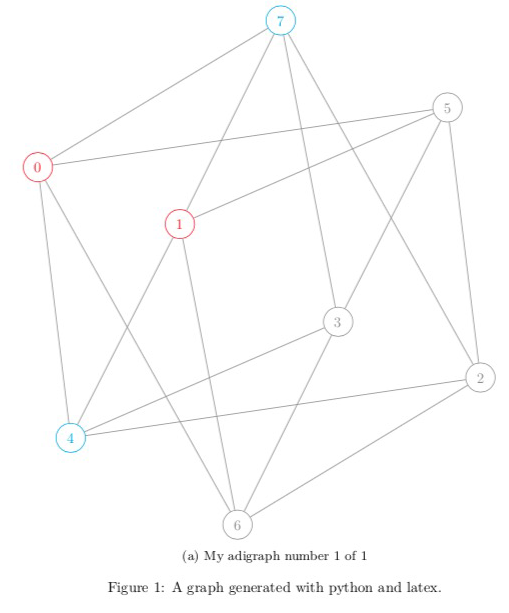
\includegraphics[width=0.5\textwidth]{img_examples/pyadigraph.png}
\end{figure}

\chapter{Warnings}
\section{Reserved words}
I reserve to use for the package the following tokens:

\begin{multicols}{2}
	\begin{enumerate}
		\item \textbackslash Adigraph
		\item \textbackslash AdigraphBuildEdge
		\item \textbackslash AdigraphBuildEdgeWrapper
		\item \textbackslash AdigraphBuildNode
		\item \textbackslash AdigraphBuildNodeWrapper
		\item \textbackslash AdigraphBuildPath
		\item \textbackslash AdigraphCalculateOrientation
		\item \textbackslash AdigraphCountPaths
		\item \textbackslash AdigraphCutBuilder
		\item \textbackslash AdigraphDrawEdge
		\item \textbackslash AdigraphDrawNode
		\item \textbackslash AdigraphEdgeBuilder
		\item \textbackslash AdigraphEdgeDrawer
		\item \textbackslash AdigraphElaboratePath
		\item \textbackslash AdigraphExecuteCutBuilder
		\item \textbackslash AdigraphGenerateNodeName
		\item \textbackslash AdigraphMemorizeEdge
		\item \textbackslash AdigraphMemorizeNode
		\item \textbackslash AdigraphNodeBuilder
		\item \textbackslash AdigraphNodeCounter
		\item \textbackslash AdigraphNodeCounterSecondWrapper
		\item \textbackslash AdigraphNodeCounterWrapper
		\item \textbackslash AdigraphNodesCounter
		\item \textbackslash AdigraphPathBuilder
		\item \textbackslash AdigraphProcessAugmentingPaths
		\item \textbackslash AdigraphProcessAugmentingPathsList
		\item \textbackslash AdigraphProcessCuts
		\item \textbackslash AdigraphProcessEdges
		\item \textbackslash AdigraphProcessNodes
		\item \textbackslash AdigraphProcessPaths
		\item \textbackslash AdigraphSimpleSum
		\item \textbackslash NewAdigraph
		\item \textbackslash RenewAdigraph
	\end{enumerate}
\end{multicols}

\end{document}